\documentclass[a4paper,10pt]{article}
\usepackage{amssymb}
\usepackage{graphicx}
\graphicspath{{../fig/}}
\usepackage{fullpage}
\usepackage{hyperref} 

\hypersetup{
bookmarks,
plainpages=false,
colorlinks=true,
pdfborder={0 0 0 0},
linkcolor=blue,
citecolor=blue,
urlcolor=blue,
pdfstartview={FitH},
bookmarksopen=false,
unicode
}

\newcommand{\src}[1]{\href{http://bitbucket.org/gkw/gkw/src/HEAD/src/#1}{#1}}
\newcommand{\doc}[1]{\href{http://bitbucket.org/gkw/gkw/src/HEAD/doc/#1}{#1}}
\newcommand{\raw}[1]{\href{http://bitbucket.org/gkw/gkw/raw/HEAD/#1}{#1}}
\newcommand{\scripts}[1]{\href{http://bitbucket.org/gkw/gkw/src/HEAD/scripts/#1}{#1}}
\newcommand{\matlab}[1]{\href{http://bitbucket.org/gkw/gkw/src/HEAD/matlab/#1}{#1}}
\newcommand{\trunk}[1]{\href{http://bitbucket.org/gkw/gkw/src/HEAD/#1}{#1}}

\setlength{\textheight}{24cm}

\newcommand{\pd}[2]{\frac{\partial #1}{\partial #2}} % for partial derivatives

%opening
\title{GKW for Beginners}
\author{F.J. Casson}
\date{11 April 2008.  Last Revised 18 Jan 2016.}
\setlength{\parindent}{0pt}

\begin{document}

\maketitle

%%%%%%%%%%%%%%%%%%%%%%%%%%%%%%%%%%%%%%%%%%%%%%%%%%%%%%%%%%%%%%%%%%%%%%%%

\begin{abstract} 

  This introductory document aims to describe the very basic things a
  newcomer needs to know in trying to understand or use GKW. These are
  the things that are mostly obvious to anyone who has worked with the
  code on any serious level.  To anyone who has worked with another
  gyrokinetic code many of these things will also be obvious, but
  there are practicalities specific to GKW.  Therefore this document
  has to be written and improved by newcomers still in the early
  stages of learning GKW.  This is still a work in progress, as such
  you are encouraged to add to and improve it.

\end{abstract}

%%%%%%%%%%%%%%%%%%%%%%%%%%%%%%%%%%%%%%%%%%%%%%%%%%%%%%%%%%%%%%%%%%%%%%%%

\tableofcontents
\setlength{\parskip}{8pt}

%%%%%%%%%%%%%%%%%%%%%%%%%%%%%%%%%%%%%%%%%%%%%%%%%%%%%%%%%%%%%%%%%%%%%%%%
\section{What does the code do?}

The code GKW solves the gyrokinetic Vlasov equation for the evolution
of plasma particle distribution functions self consistently with the
Maxwell equations in a toroidally symmetric geometry. More precisely,
it solves it only for the perturbation $f$ of an equilibrium
distribution $F_M$ (also called the background), similar to an Ansatz
in linear perturbation theory.
\begin{equation}
  f_{tot} = F_M + f
\end{equation}

One important idea of the gyrokinetic model is that one velocity
dimension of the general Vlasov equation is removed by averaging over
the small scale cyclotron (gyro) motion of a charged particle in a
magnetic field. Thus the equations are 5 dimensional (3 space, 2
velocity) with the two directions of velocity $\mu$ (the magnetic
moment, being connected to $v_\perp$) and $v_\parallel$.  This
simplification by one dimension makes a numerical simulation of
microscale plasma turbulence tractable.

For the purpose of simulation a tokamak core plasma, the field aligned Hamada coordinate system is
introduced, which separates the directions parallel and perpendicular to the
magnetic field. This allows to apply the following assumptions, called the
'gyrokinetic ordering': One assumes certain length
scales for parallel and perpendicular derivatives of distribution and
field perturbations.
\begin{equation}
\nabla_\parallel  \sim \frac{1}{R} \quad \mathrm{and}\quad
\nabla_\perp \sim \frac{1}{\rho_{ref}} =  \frac{1}{R}\frac{R}{\rho_{ref}} = \frac{1}{R\rho_*}
\end{equation}
where $R$ is a typical length scale of the background (like the
tokamak major radius) and $\rho_{ref}$ is a typical gyroradius. The
ratio $\rho_*=\rho_i/R$ is a small number, serves as a smallness
parameter in this model and appears also in an assumption called the
$\delta f$-approximation:
\begin{equation}
  f \sim \rho_*F_M\quad\mathrm{and}\quad \pd{f}{v_\parallel}\sim\rho_*
\end{equation}

When constructing a gyrokinetic equation including terms of at most (say) first
order in $\rho_*$, these assumption about the structures of interest
allow to neglect certain terms, e.g. such containing parallel derivatives
of perturbed quantities.

Hence, these orderings mean that the model will resolve and include structures
perpendicular to the magnetic field on the scale of the Larmor radius
$\rho_i$, whilst parallel structures will have a length scale of the
order of the system (tokamak) size $R$. This ordering is chosen to
describe drift wave structures.

The GKW code has a number of useful features, such as the ability
to model many plasma species, including non linear terms, kinetic
electrons, particle collisions, a rotating plasma and arbitrary flux
surface geometry (through interface with the CHEASE code),
tearingmodes and others.

%%%%%%%%%%%%%%%%%%%%%%%%%%%%%%%%%%%%%%%%%%%%%%%%%%%%%%%%%%%%%%%%%%%%%%%%
\section{Where is the code?}

In the git repository at bitbucket.  Non-members may clone a read-only working copy anonymously over HTTP.  

\texttt{git clone git@bitbucket.org:gkw/gkw.git}.

Some additional git workflow guidance for GKW is on the \href{https://bitbucket.org/gkw/gkw/wiki/Git_Bitbucket}{wiki}.
If you have not used git before then briefly read: Chapters 1 and 2 of the git book (\href{http://git-scm.com/book/en/v2}{http://git-scm.com/book/en/v2}).  Bitbucket has a graphical user interface which makes it easy to use many of the features of git.

When you check out the code the following folders will be created:
\begin{itemize}
 \item \texttt{/src} contains all the source code for GKW.
 \item \texttt{/doc} contains documentation files. \texttt{/doc/input} contains some sample input files.
 \item \texttt{/config} contains build configuration makefiles for some hosts
 \item \texttt{/tests} contains a set of test cases we use for testing changes made to the code.
 \item \texttt{/matlab} contains matlab scripts for preparing input files and interpreting output data.
 \item \texttt{/octave} contains GNU Octave scripts for preparing input files and interpreting output data.
 \item \texttt{/python} contains Python scripts for handling output data.
 \item \texttt{/scripts} contains various scripts which (amongst other
   things) can compile GKW from any working directory
   (\texttt{gkwmake}), can check if the code is working as it should
   (\texttt{gkw\_run\_tests}), delete all output files of a GKW run
   (\texttt{gkw\_clean\_run}), start a simulation locally with the
   newest executable (\texttt{gkwrun}) or submit multiple jobs
   (\texttt{gkwnlin}). See their help messages or instruction at the
   beginnig of these scripts.
 \item \texttt{/libs} contains additional libraries that are needed
   and also provided with gkw for easier compilation.
\end{itemize}

It is required by various scripts that you define a \texttt{GKW\_HOME}
environment variable which is the path to your GKW folder, as this
variable is used in some scripts. Adding the following to your
\texttt{.bashrc} file will make these things automatic:

\begin{verbatim}
   export GKW_HOME="/path/to/gkw/"
   export PATH="$PATH:${GKW_HOME}/scripts"
\end{verbatim}

%%%%%%%%%%%%%%%%%%%%%%%%%%%%%%%%%%%%%%%%%%%%%%%%%%%%%%%%%%%%%%%%%%%%%%%%
\section{How do I compile from source?}

The code should compile with default options on your machine by running \texttt{gkwmake -j} (or \texttt{gmake} in the top level GKW directory). This will create:
\begin{itemize}
\item \texttt{/obj} folder for all the object files (these can be deleted later)
\item \texttt{/run} folder which will contain the compiled executable. 
\end{itemize}

On many shared machines, GKW makefiles are already configured.  
When you build for the first time on a new machine, a template configuration file will be created for your machine in \textit{./config/machine}.  
The basic configuration will not contain MPI or FFTW (needed for parallel or nonlinear runs).
You can configure FFTW and MPI and other compile options specific to your machine by editing the file \textit{default.mk} in this folder. 
\texttt{gkwmake clean} will remove all the object files if you want to do a completely fresh compile.

While developing new code it is strongly recommended to compile with
\begin{verbatim}
   gkwmake -j DEBUG=on OPTFLAGS=off
\end{verbatim}
whereas executables for production runs will become optimised for speed with
\begin{verbatim}
   gkwmake -j DEBUG=off OPTFLAGS=on
\end{verbatim}

\section{How do I do a run?}

You need to create a file named \texttt{input.dat} in the same
directory as the executable.  This file is the input deck containing
all the switches which control how the code runs.  There are some
sample input files in \texttt{/doc/input}. Also in the \texttt{/doc}
folder is an \doc{input.dat.sample} file which should briefly describe
all the input variables. Many of the input switches are optional and
default values will be used if they are not provided.  The
\doc{input.dat.minimum} file shows the variables that \textit{must} be
provided.

The code is quite sensitive to bad formatting or typos in
\texttt{input.dat}, in which case you will hit a read error as soon as
you run the code.  Most of the time if you input a set of incompatible
switches the code will tell you and throw you out.

Two key output files created are \texttt{time.dat} which records the
(linear) mode growth rate against time, and \texttt{fluxes.dat} which
records particle fluxes against time.  More details on the other
output files are in the main manual.

A few salient points about the input file (many more in the full
manual):

\subsection{Output File Format}
The setting of \texttt{io\_format} controls if diagnostic data is
output as HDF5 file or as many ASCII or binary files. The setting
\texttt{io\_legacy} switches between historically grown data ordering
and a more cleaned-up ordering (e.g. data in form of a long flat
column vs. a n-dimensional matrix)\\
In the long run, it is recommended to use
\texttt{io\_format=hdf5+ascii} and \texttt{io\_legacy=F}.

\subsection{Species}
There is no default species data, hence you must provide some. The species you input must satisfy quasi-neutrality. This requires you to set ratios of densities and charge appropriately such that the sum over all species $s$ is zero:
\begin{equation}
 \sum_s z_s \cdot dens_s = 0
\end{equation}
\begin{equation}
 \sum_s z_s \cdot dens_s \cdot rln_s= 0
\end{equation}
You can input multiple ion species but only one negatively charged species (electrons) is allowed.  Note that the number of species read in is controlled by the number of species parameter in the 'gridsize' namelist and hence it is possible that later species data you specify will not be read in if this is set incorrectly.  The \texttt{number\_of\_species} input variable does not include adiabatic electrons but the species data for these will still be read if this the case.

\subsection{Timestep and resolution}
The timestep required for stability can vary greatly depending on input parameters or choice of scheme.  In particular kinetic electrons require a timestep $10^{-2}$ smaller.  The question of necessary resolution needed is even harder to answer, in fact it is one of the controversial questions in gyrokinetics.  To a large extent it depends on which physics problem you want to study.  Use the sample provided \doc{input} files to get you started.

\subsection{Parallelisation}
To run parallel (MPI) jobs you need to be in an environment which
provides the an MPI library and with an mpi controller configured and
running. It may help to execute \texttt{type mpiexec} or \texttt{type
  mpirun}, or \texttt{gkw\_run\_tests --parallel} to see if this is the
case.

If the parallelisation scheme is not explicitely given in the input
file via the \texttt{n\_procs\_*} parameters the code will select what
it considers to be the most appropriate parallelisation given your
computational grid.  The code will parallelise first
over the $\mu$ grid and (non-adiabatic) species, and then over the
$v_{\parallel}$ and $s$ grid points.  Nevertheless it is sensible to
have in mind a parallelisation setup when you set the gridsize, as the
user controls the number of processors the code will be run on and
should choose a number that fits with the gridsize.

\subsection{Modes}
The spacing and location of the modes is determined by the `modes' namelist.   For linear runs, set \texttt{mode\_box=.false.}, \texttt{NX=1} and \texttt{NMOD=1}.  For nonlinear runs, there is a spreadsheet \doc{mode\_box\_calculator.ods} in the documentation folder which should help you determine the mode spacing.

\subsection{Solver Methods}
Safest option:
\begin{verbatim}
METHOD='EXP'
METH=2
\end{verbatim}

\subsection{Batch jobs}
There are also scripts for doing multiple runs. The script \scripts{gkwnlin}  uses a directory structure with batch input files all put in an input folder (with different names), and output files will all be put in relevant folders.  The scripts submit jobs to a queue in the portable batch system (PBS).  If you haven't used PBS before, read a little about how it works.

Typical workflow for a batch job is the following:
\begin{itemize}
\item Compile the GKW executable for the machine you are on. 
\item Run \texttt{gkwnlin -p project\_name} to create a new project directory.
\item Run matlab script \matlab{create\_gkwscan} to make a scan of the given input file and put these in the input folder.  Or if you only need to make a few input files, you can do this manually.
\item Run \texttt{gkwnlin} from the input folder to submit multiple input files to the PBS queue.  Use something like \texttt{gkwnlin -np 8 -h 3 *}.  gkwnlin will take the most recent executable from \texttt{\$GKW\_HOME/run} to run with all the input files you give. 
\item Run \texttt{qstat} to the status of your jobs in the queue and see if they are running yet.
\item After the first loop has completed you should look in the output files ./runs/*/out, to check the job is running ok.
To stop an individual job use \texttt{qdel}, or do \texttt{touch gkw.stop} in its run folder for a clean stop.
\item Go get coffee.

\end{itemize}

These scripts are self documenting on the -options syntax they require.  Type \texttt{gkwnlin} for help, or in matlab \texttt{help create\_gkwscan}.  Note that \texttt{create\_gkwscan} works best if you keep your batch projects runs in \texttt{~/runs/gkw/}; or else reconfigure the matlab script \texttt{gkwpath}.

\section{Geometry and Domain}

\begin{figure}[hb!]
 \begin{center}
 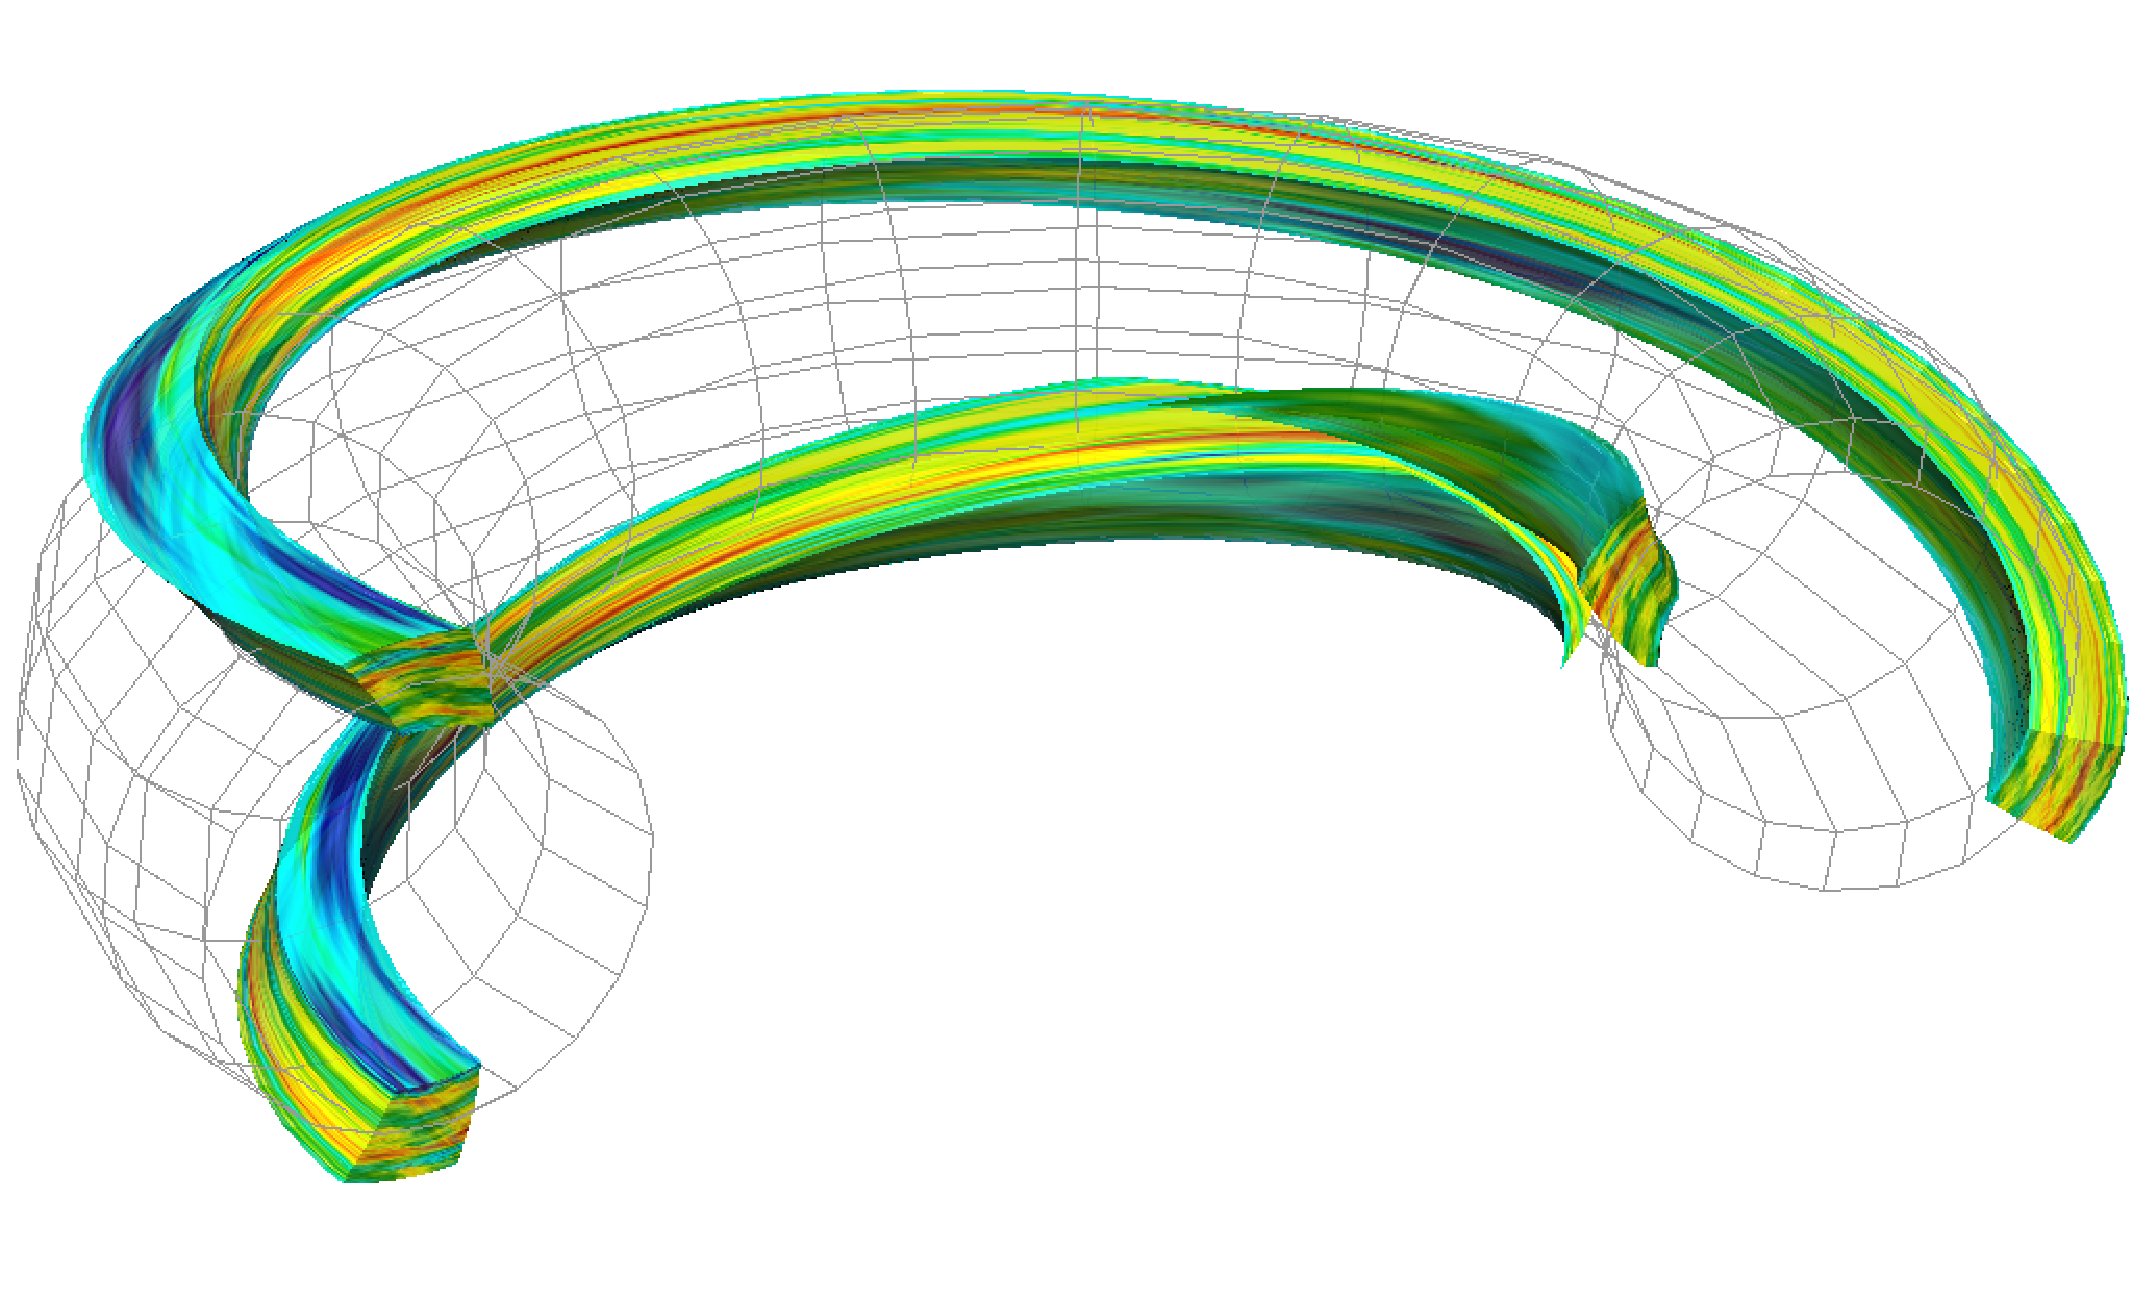
\includegraphics[scale=0.3]{flux_tube.eps}
\caption{Sketch of the flux tube domain with $q=2$, $\epsilon=r/R=0.29$ and $\hat{s}=1$ showing the GKW coordinate directions.} 
 \label{fig.domain}
\end{center}
\end{figure}

\begin{figure}[ht!]
 \begin{center}
 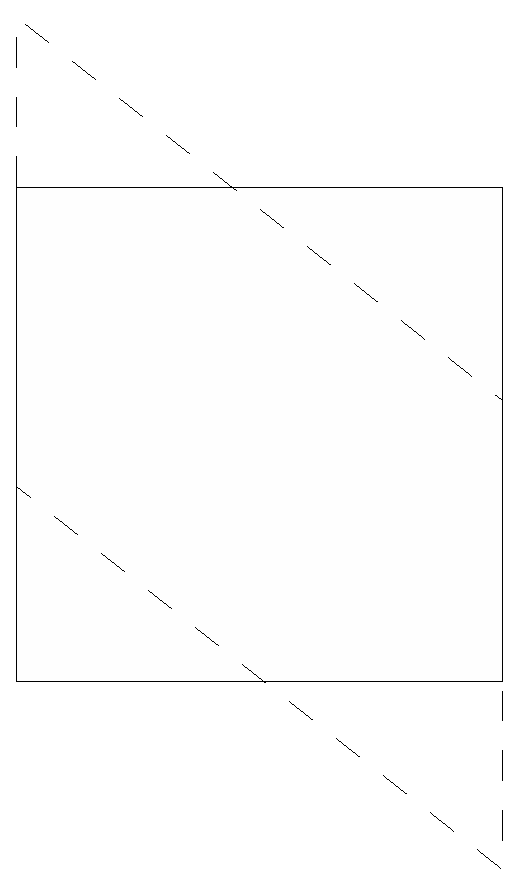
\includegraphics[scale=0.3]{shear.eps}
\caption{Superposition of two perpendicular cross sections of the flux tube separated by one polodial circuit.  The flux tube is sheared as it follows the magnetic shear.  This picture hopes to make clear that each $k_\zeta$ mode must connect to a higher one for a periodic boundary in $s$.  Namely, the difference between connected modes is $\Delta k_\psi = k_\zeta {\partial q \over \partial \psi}$. }
 \label{fig.shear}
\end{center}
\end{figure}

The coordinates used are field aligned Hamada coordinates $(s, \psi, \zeta)$,  in which magnetic field lines are straightened. In these coordinates, the components of the magnetic field are flux functions and $B^\psi = B^\zeta = 0$ so that ${\bf B} \cdot \nabla = B^s {\partial \over \partial s}$.  Whilst $s(\theta,\phi)$ is a coordinate along the field line, $\psi(r)$ is a radial coordinate which describes the flux surfaces and $\zeta(\theta,\phi)$ is a (mostly poloidal) coordinate which lies within a flux surface.  The purpose of these coordinates is to allow separation of the different length scales of the parallel and perpendicular plasma dynamics.

GKW is written with general tensors so that in principle the code can deal with any toroidally symmetric 
equilibrium. This means that all the equations are expressed with the use of general tensors, and 
the metric elements. Currently  the geometry dependent quantities are calculated in the code only for the $\hat s - \alpha$ equilibrium. In addition, GKW can read CHEASE output for arbitrary flux surface configuration. CHEASE takes an input of the shape of the last closed flux surface, a boundary pressure, and a current profile. From these inputs, CHEASE solves the Grad-Shafranov equation to find an equilibria flux surface configurations which it outputs as the poloidal flux. See the documentation file \texttt{gkwandchease.tex} for more information.

GKW is a local gyrokinetic code modelling a flux tube domain, and is spectral (with periodic boundaries) in both directions perpendicular to a field line.  The flux tube domain is bounded by four magnetic field lines, two within each of two adjacent flux surfaces (Fig \ref{fig.domain}). As the domain progresses helically round the torus it is sheared with the magnetic shear.  When one poloidal circuit is completed the flux tube can be connected to itself, but the shear requires the $k_\psi$ modes to be be connected (Fig. \ref{fig.shear}) at the $s$ boundary.

In GKW, computation in the perpendicular directions is done in the wavevector domain for computational efficiency, whilst a finite difference scheme is used in the parallel directions.  In the general formulation, this pseudo-spectral method is more general than assuming an eikonal form for the solution. In our ordering of terms we keep only first order terms in $\rho_*=\rho/R \ll 1$, which makes the two approaches equivalent.  The transformation to field aligned coordinates is mathematically equivalent to the ballooning transform of the eikonal form in this case. The periodicity constraints equate to the coupling of the $k_\psi$ modes described above.  Since the flux tube is sheared, the consequences of magnetic shear is to couple the modes.  For further details see the section \textit{local limit} in \textit{GKW How and Why}.

\section{What is under the bonnet?}

The code is written in Fortran 95 and uses MPI for (optional) parallel implementation.  The code is split into separate Fortran modules in the \texttt{src} folder.  The program runs from \texttt{gkw.f90} and then uses the modules as called from there, each of which can recursively call other modules. 
The automatically generated reference dictionary for the code is at \href{http://www.gkw.org.uk/doxygen}{http://www.gkw.org.uk/doxygen} and is a useful way to explore the code.   The file \texttt{program\_flow} in the documentation folder shows the code progression (though it is a little out of date).
If you want to familiarise yourself with inner details of the code, we suggest that after reading the manual, you look at the source files 
\src{gkw.f90}, \src{init.f90}, \src{mode.f90}, \src{linear\_terms.F90} and \src{exp\_integration.F90}, in that order.

\begin{itemize}
\item Modules *.F90 are put through the preprocessor mainly for processing \#if blocks for MPI.
\item Modules *.f90 are not put through the preprocessor.
\end{itemize}

\section{Philosophy behind the coding}

\begin{itemize}
 \item The code is designed to make initialisation procedures easy to read.  As such they may not be the most computationally efficient ways of doing things. Only the computationally expensive parts of the code are optimised, other parts are designed to be readable.

 \item The code has a lot built in error reporting with the idea that if you break something, or if something is currently not working, it will tell you.  In addition, the script \scripts{gkw\_run\_tests} will run the code against a set of test cases and report if any changes made have altered the physics output of the code.

 \item The code uses global variables for most things.  This is a compromise with simplicity and readability by reducing the need for functions with many arguments passed to them. 
To avoid confusing problems often associated with global variables the \texttt{use control,only : number of processors} and data hiding within modules limits the use of variables declared in other modules to those explicitly named.

\end{itemize}

\section{Checking in changes to the code}

If you are going to contribute changes to the code, you will need a bitbucket.org account and your username will need to be added to the list of authorised users.  More details can be found on the \href{https://bitbucket.org/gkw/gkw/wiki/Git_Bitbucket}{GKW wiki}.

Think carefully before you push something as it will be visible for all the world to see, forever.  Do not commit any code that is not open source.  The repository should only be used for plain text files (and possibly some small figures).  Before you push any changes to the source, you should run the test script \texttt{gkw\_run\_tests} to check you have not broken the code.  This script runs the code under a number of scenarios and checks if the physics output has changed relative to a previously generated reference output.

When committing (\texttt{git commit}) you should specify a log message, for which a text editor will open.  This message is stored in the Git log. The first line should be a brief summary, followed by a blank line, followed by the details.   The default text editor can be changed by putting (for example) \texttt{export EDITOR=kwrite} in your \texttt{.bashrc}.

\section{Where can I get more help?}

The following are other useful GKW resources.

\begin{itemize}
\item The GKW manual at \href{http://www.gkw.org.uk/tikiwiki/Manual}{http://www.gkw.org.uk/tikiwiki/Manual} has a detailed description of the gyrokinetic framework as is implemented in GKW covering the equations, co-ordinate system, and normalisations of the code.  It also includes further details on running the code, input and output files, and the benchmarks.

\item A full listing of all the input variables is provided in \doc{input.dat.sample}

\item An automatically generated reference dictionary for the code is at 
\href{http://www.gkw.org.uk/doxygen}{http://www.gkw.org.uk/doxygen}

\item Browse some of the papers in which GKW has been used to get an idea of what it does.

\href{http://www.gkw.org.uk/tikiwiki/publications}{http://www.gkw.org.uk/tikiwiki/publications}

\item The wiki at \href{https://bitbucket.org/gkw/gkw/wiki}{https://bitbucket.org/gkw/gkw/wiki}.

\item If you find a problem with code, please submit it to the issue tracker: 

\href{https://bitbucket.org/gkw/gkw/issues}{https://bitbucket.org/gkw/gkw/issues}

\item Arthur Peeters obviously knows the answer to most GKW questions, but other people working with the code may know the answer to simple questions, just ask.  

\end{itemize}

\end{document}
